\section{Divisibility}\label{sec:divisibility}
%% FUNCTION: Shows how the EFX rate of round robin changes with the remainder q at three goods per
%% agent (m = 12 to 15 for n = 4). Divisibility decides when values are similar and fades when
%% values are very unequal, which is why the main figure shows three levels of dispersion. With
%% identical valuations and q > 0, round robin is never EFX (proven).

\subsection{EFX Rate}\label{sec:divisibility-rate}

\begin{figure}[H]
  \centering
  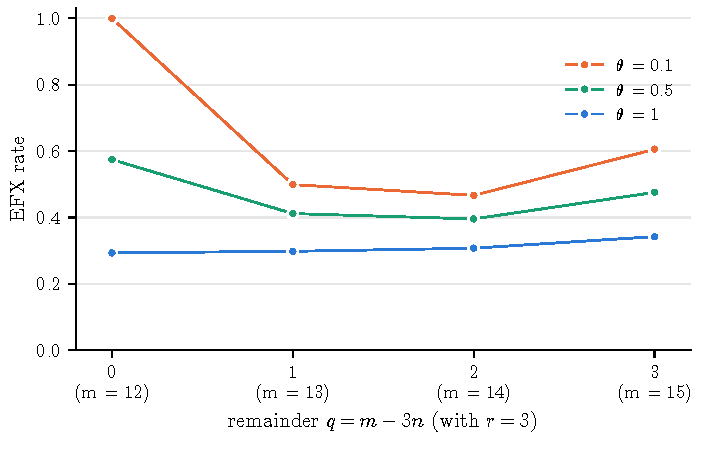
\includegraphics{fig44_divisibility_rate.pdf}
  \caption{EFX rate of Round Robin against the remainder $q$, for $n=4$ agents with $r=3$ goods per agent
  ($m=12$ to $15$) and agreement $\rho=0.5$, one line per level of dispersion $\theta$. Each
  point rests on $R=20{,}000$ instances. The lines between the points are for illustration only.}
  \label{fig:divisibility}
\end{figure}

\subsection{Identical Valuations without Divisibility}\label{sec:divisibility-identical}

\subsection{Severity of Failures}\label{sec:divisibility-severity}

\begin{figure}[H]
  \centering
  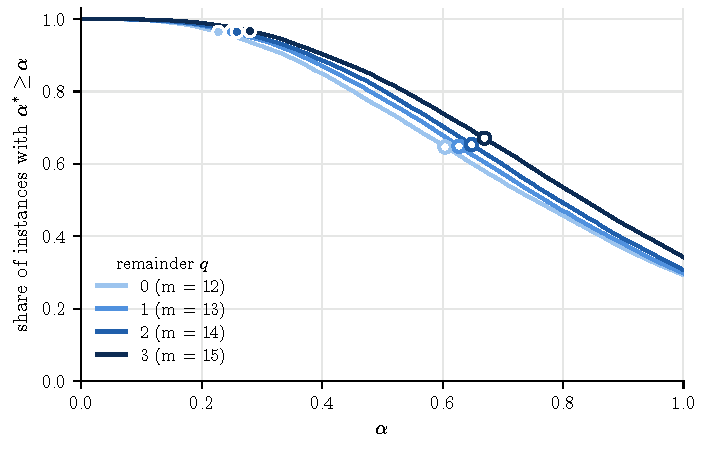
\includegraphics{fig44_divisibility_survival.pdf}
  \caption{Share of instances with $\astar\geq\alpha$ under Round Robin, one curve per remainder $q$, for
  $n=4$ agents with $r=3$ goods per agent ($m=12$ to $15$), agreement $\rho=0.5$ and dispersion
  $\theta=1$. Each curve rests on $R=20{,}000$ instances. The filled point on each curve marks
  the $5\%$ quantile and the open point the median of $\astar$ among the instances that are not
  EFX.}
  \label{fig:divisibility-survival}
\end{figure}

